\documentclass[11pt]{article}
\usepackage[paper=a4paper,top=1.5cm,left=1.5cm,right=1.5cm,
    foot=1cm,bottom=1.5cm]{geometry}

\usepackage{times}
\usepackage[T1]{fontenc}
\usepackage[utf8]{inputenc}
\usepackage[english,russian]{babel}
\usepackage{amssymb,amsfonts,amsmath,mathtext,amsbsy}
\usepackage{multirow}
\usepackage{listings}
\usepackage{graphicx}
\graphicspath{{./images/}}

\newcommand{\comment}[1]{}
\newcommand{\br}[1]{\boldsymbol{\mathrm{#1}}}
%\newcommand{\br}[1]{\bm{\mathrm{#1}}}

\newenvironment{packed_enum}{
\begin{enumerate}
  \setlength{\itemsep}{1pt}
  \setlength{\parskip}{0pt}
  \setlength{\parsep}{0pt}
}{\end{enumerate}}

\title{VVHD}
\author{Я. А. Дынников}

\begin{document}

\maketitle

%%%%%%%%%%%%%%%%%%%%%%%%%%%%%%%%%%%%%%%%%%%%%%%%%%%%%%%%%%%%%%%%%%%%%%%%%%%%%%%%
\begin{abstract}
Это мануал, посвященный исходникам библиотеки. Здесь я постараюсь 
описать его структуру, способы работы с ним, и подводные камни, 
на которые нужно будет обращать внимание.
\end{abstract}

\section{TList}
Лист является шаблонным классом и надстройкой над массивом. 
Лист предоставляет функции добавления, удаления элементов и 
динамического изменения размеров. В принципе, лист является 
усовершенствованным вектором (из std::), он даже почти полностью
с ним совместим.

\lstset{language=C++, frame=single}
\begin{lstlisting}
template <class T>
class list
{
	public:
		list();
		~list();

		void push_back(const T &item);
		void erase(T* item);
		void clear();
		T& at(size_t i);
		T* begin();
		T* end();
		size_t size();
		size_t size_safe();
		T* next(T* item);
		T* prev(T* item);

	private:
		size_t size_;
		size_t maxsize;
		T* begin_;
		T* end_;

		void realloc_();
};

#define const_for(list, it) \
	for (auto it=list->begin(); it<list->end(); it++)
\end{lstlisting}

Вот о чем нужно помнить
\begin{enumerate}
\item Если вы добавляете в массив элементы, не пользуйтесь 
инкрементом TObj* obj++. Если вдруг произойдет realloc ---
адресация массива сменится непредсказуемо.
\item При удалении элемента на его место перемещается последний 
элемент, а size уменьшается.
Если Вы удалили элемент функцией erase(), не забудте указатель
уменьшить на единичку, иначе этот элемент массива останется необработанным
\end{enumerate}

%%%%%%%%%%%%%%%%%%%%%%%%%%%%%%%%%%%%%%%%%%%%%%%%%%%%%%%%%%%%%%%%%%%%%%%%%%%%%%%%
\section{Convective}
\subsection{ConvectiveInfluence}
Функция вычисляет интеграл скорости, индуцируемый единичным вихрем 
в точке $\br p$ на отрезок $[\br p_1, \br p_2]$
В комплексных переменных координаты следующие:
$z = p_x - i p_y$, $z_c = \frac{1}{2}(z_1 + z_2)$


\begin{equation*}
\int\limits_{z_1}^{z_2} \left (\br V \cdot d \br S \right ) = 
\begin{cases}
-\Re \left\lbrace \log \left(\dfrac{z-z_1}{z-z_2}\right) \right\rbrace,	&\text{для дальних}\\
\dfrac{1}{\varepsilon^2}\Re \left\lbrace (z_c-z)(\bar z_2 - \bar z_1) \right\rbrace, 	&\text{для ближних}\\
\end{cases}
%записать по русски условия
\end{equation*}
\begin{center}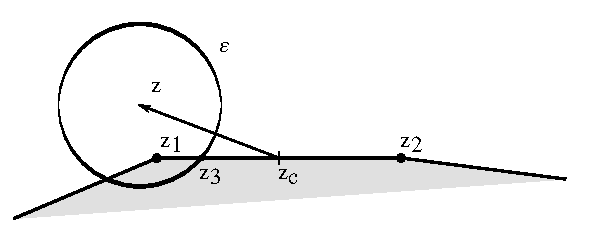
\includegraphics{ConvInfluence.pdf}\end{center}

Если один из концов отрезка является ближним, а другой дальним, 
отрезок делится на две части точкой $\br p_3$, для каждой
из которых влияние вычисляется по своей формуле.
В обычном случае, функцию для блихних вихрей удобней записать без использования
комплексных чисел:
$(\br p_c - \br p)(\br p_2 - \br p_1 ) / \varepsilon^2$

%%%%%%%%%%%%%%%%%%%%%%%%%%%%%%%%%%%%%%%%%%%%%%%%%%%%%%%%%%%%%%%%%%%%%%%%%%%%%%%%
\newpage
\section{Diffusive}
\subsection{Vortex diffusive}

$\br r$ - координаты текущего вихря (для которого вычисляем скорость) \\
$\br V_d$ - диффузионная скорость текущего вихря, индуцированная другими вихрями \\
$\varepsilon$ - расстояние от текущего вихря до 2го ближайшего \\
$\br r_j, \gamma_j$ - координата j-го вихря и его циркуляция \\
$\br\rho_j = \br r - \br r_j$ - и так понятно \\

\begin{equation*}
\br V_d = -\dfrac{1}{\text{Re}} \dfrac{1}{\varepsilon} 
\dfrac{\sum\limits_j (\br\rho_j / \lvert\rho_j\rvert)\cdot\gamma_j e^{-\lvert\rho_j\rvert/\varepsilon}}
{\sum\limits_j \gamma_j e^{-\lvert\rho_j\rvert/\varepsilon}}
\end{equation*}

\begin{center}\setlength\fboxsep{0pt}
\setlength\fboxrule{0.5pt}
\fbox{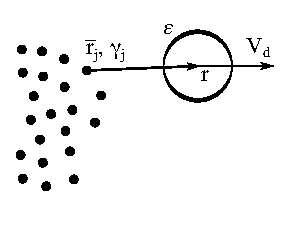
\includegraphics{VortexDiff.pdf}}
\end{center}

%%%%%%%%%%%%%%%%%%%%%%%%%%%%%%%%%%%%%%%%%%%%%%%%%%%%%%%%%%%%%%%%%%%%%%%%%%%%%%%%
\subsection{Body diffusive}

$\br r$ - координаты текущего вихря (для которого вычисляем скорость) \\
$\br W_d$ - диффузионная скорость текущего вихря, индуцированная стенкой \\
$\br p_k$ - k-я вершина тела \\
$\br r_k = \frac{1}{2}(\br p_k + \br p_{k+1})$ - центр k-го отрезка тела \\
$d \br S_k = \br n \cdot\lvert\br p_{k+1} - \br p_k \rvert$ - нормаль к k-му отрезку, с длиной, равной длине отрезка \\
$\br{\rho}_k = \br r - \br r_k$ - и так понятно \\

\begin{equation*}
\br W_d = -\dfrac{1}{\text{Re}} \dfrac{1}{\varepsilon^2} 
\dfrac{\sum\limits_k d\br S_k\cdot e^{-\lvert\rho_k\rvert/\varepsilon}}
{2\pi - \sum\limits_k \dfrac{\lvert\rho_k\rvert /\varepsilon +1}{\rho_k^2}
\cdot(\br\rho_k \cdot d\br S_k)\cdot e^{-\lvert\rho_k\rvert/\varepsilon}}
\end{equation*}

\begin{center}\setlength\fboxsep{0pt}
\setlength\fboxrule{0.5pt}
\fbox{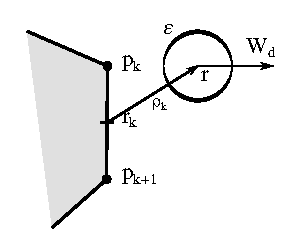
\includegraphics{BodyDiff.pdf}}
\end{center}

%%%%%%%%%%%%%%%%%%%%%%%%%%%%%%%%%%%%%%%%%%%%%%%%%%%%%%%%%%%%%%%%%%%%%%%%%%%%%%%%
\subsection{Ограничения $\br V_d$ и $\varepsilon$}
Модуль числителя $\br V_d$ не должен превышать 100 (идиотизм)\\
Если знаменатель $\br V_d$ и $\gamma_j$ (текущего) разных 
знаков --- заменяем знаменатель на циркуляцию\\
Для $\varepsilon$ --- ограничение снизу $\varepsilon > \langle dS_k \rangle$

%%%%%%%%%%%%%%%%%%%%%%%%%%%%%%%%%%%%%%%%%%%%%%%%%%%%%%%%%%%%%%%%%%%%%%%%%%%%%%%%
\newpage
\section{FlowMove}
\subsection{Схема Эйлера (классика)}
\begin{equation*}\begin{split}
&\dot{\br r} = \br V (\br r, t) \\
\Rightarrow~&\br r_{i+1} = \br r_i + \br V(\br r_i, t_i) \cdot \Delta t
\end{split}\end{equation*}

\subsection{Схема Эйлера с пересчетом}
\begin{equation*}\begin{split}
&\dot{\br r} = \br V (\br r, t) \\
\Rightarrow~&\tilde{\br r}_{i+1} = \br r_i + \br V(\br r_i, t_i) \cdot \Delta t \\
\Rightarrow~&\br r_{i+1} = \br r_i + 
\frac{\br V(\br r_i, t_i) + \br V( \tilde{\br r}_{i+1}, t_{i+1})}{2}\cdot \Delta t \\
\end{split}\end{equation*}
А что бы не хранить 2 скорости (или старые координаты) для
каждой частицы, да и вообще упростить работу с модулем,
последюю формулу перепишем в виде
\begin{equation*}
\Rightarrow~\br r_{i+1} = \tilde{\br r}_{i+1} + 
\left( -\br V(\br r_i, t_i) + \br V( \tilde{\br r}_{i+1}, t_{i+1}) \right)\cdot \frac{\Delta t}{2} \\
\end{equation*}

\subsection{Последовательность действий}
\begin{packed_enum}
\item ГУ не выполнены\\
\item Строим дерево
\item Берем скорости набегающего потока итд, заполняем СЛАУ
\item Решаем СЛАУ
\item Удаляем дерево\\
\item Сохраняемся: вихри, тела
\item Спускаем вихри, чернила, тепло\\
\item Строим дерево
\item Считаем эпсилоны, объединяем вихри
\item Считаем скорости: Convective, Diffusive, Boundary; скорости чернил, тепла
\subitem Опционально: двигаем на пол шага, заменяем скорости на отрицательные.
\subitem Опционально: считаем вторую половину скоростей.
\item Двигаем вихри, тела, стриклайны; удаляем проникшие внутрь.
\item Печатаем файл stepdata
\item $t += \Delta t$
\end{packed_enum}

%%%%%%%%%%%%%%%%%%%%%%%%%%%%%%%%%%%%%%%%%%%%%%%%%%%%%%%%%%%%%%%%%%%%%%%%%%%%%%%%
\newpage
\section{Устойчивость и выбор параметров расчета}
Согласно статье в ЖВМ, параметры расчета выбираются исходя из
соображений устойчивости. Параметрами, которые мы можем менять, являются:
$N$ --- число отрезков разбиения контура;\\
$\varepsilon_{min}$ --- ограничение на эпсилон из диффузии;\\
$\Delta t$ --- шаг по времени;\\
$r_d$ --- радиус дискретности, он же эпсилон в конвективной скорости.\\

Дополнительные обозначения:\\
$\Delta l_i$ --- длина i-го отрезка на теле, соответственно \\
$\langle\Delta l \rangle=\dfrac{1}{N} \sum\limits_{i=0}^{N} \Delta l_i$ ---
средняя длина отрезков.\\
$N$ обычно выбирается на глаз.\\
$\varepsilon_{min}=0.6\cdot\langle\Delta l \rangle$ --- 
определено в модуле diffmergefast\\
$\Delta t = \text{Re} \varepsilon_{min}^2 < 2 \text{Re} \varepsilon^2$\\
$r_d = ?$ --- а этот вопрос остается открытым \\

\end{document}
